
\begin{figure*}[!h]
    \centering
    %\includegraphics[width=1.0\linewidth]{figure/overview.pdf}
    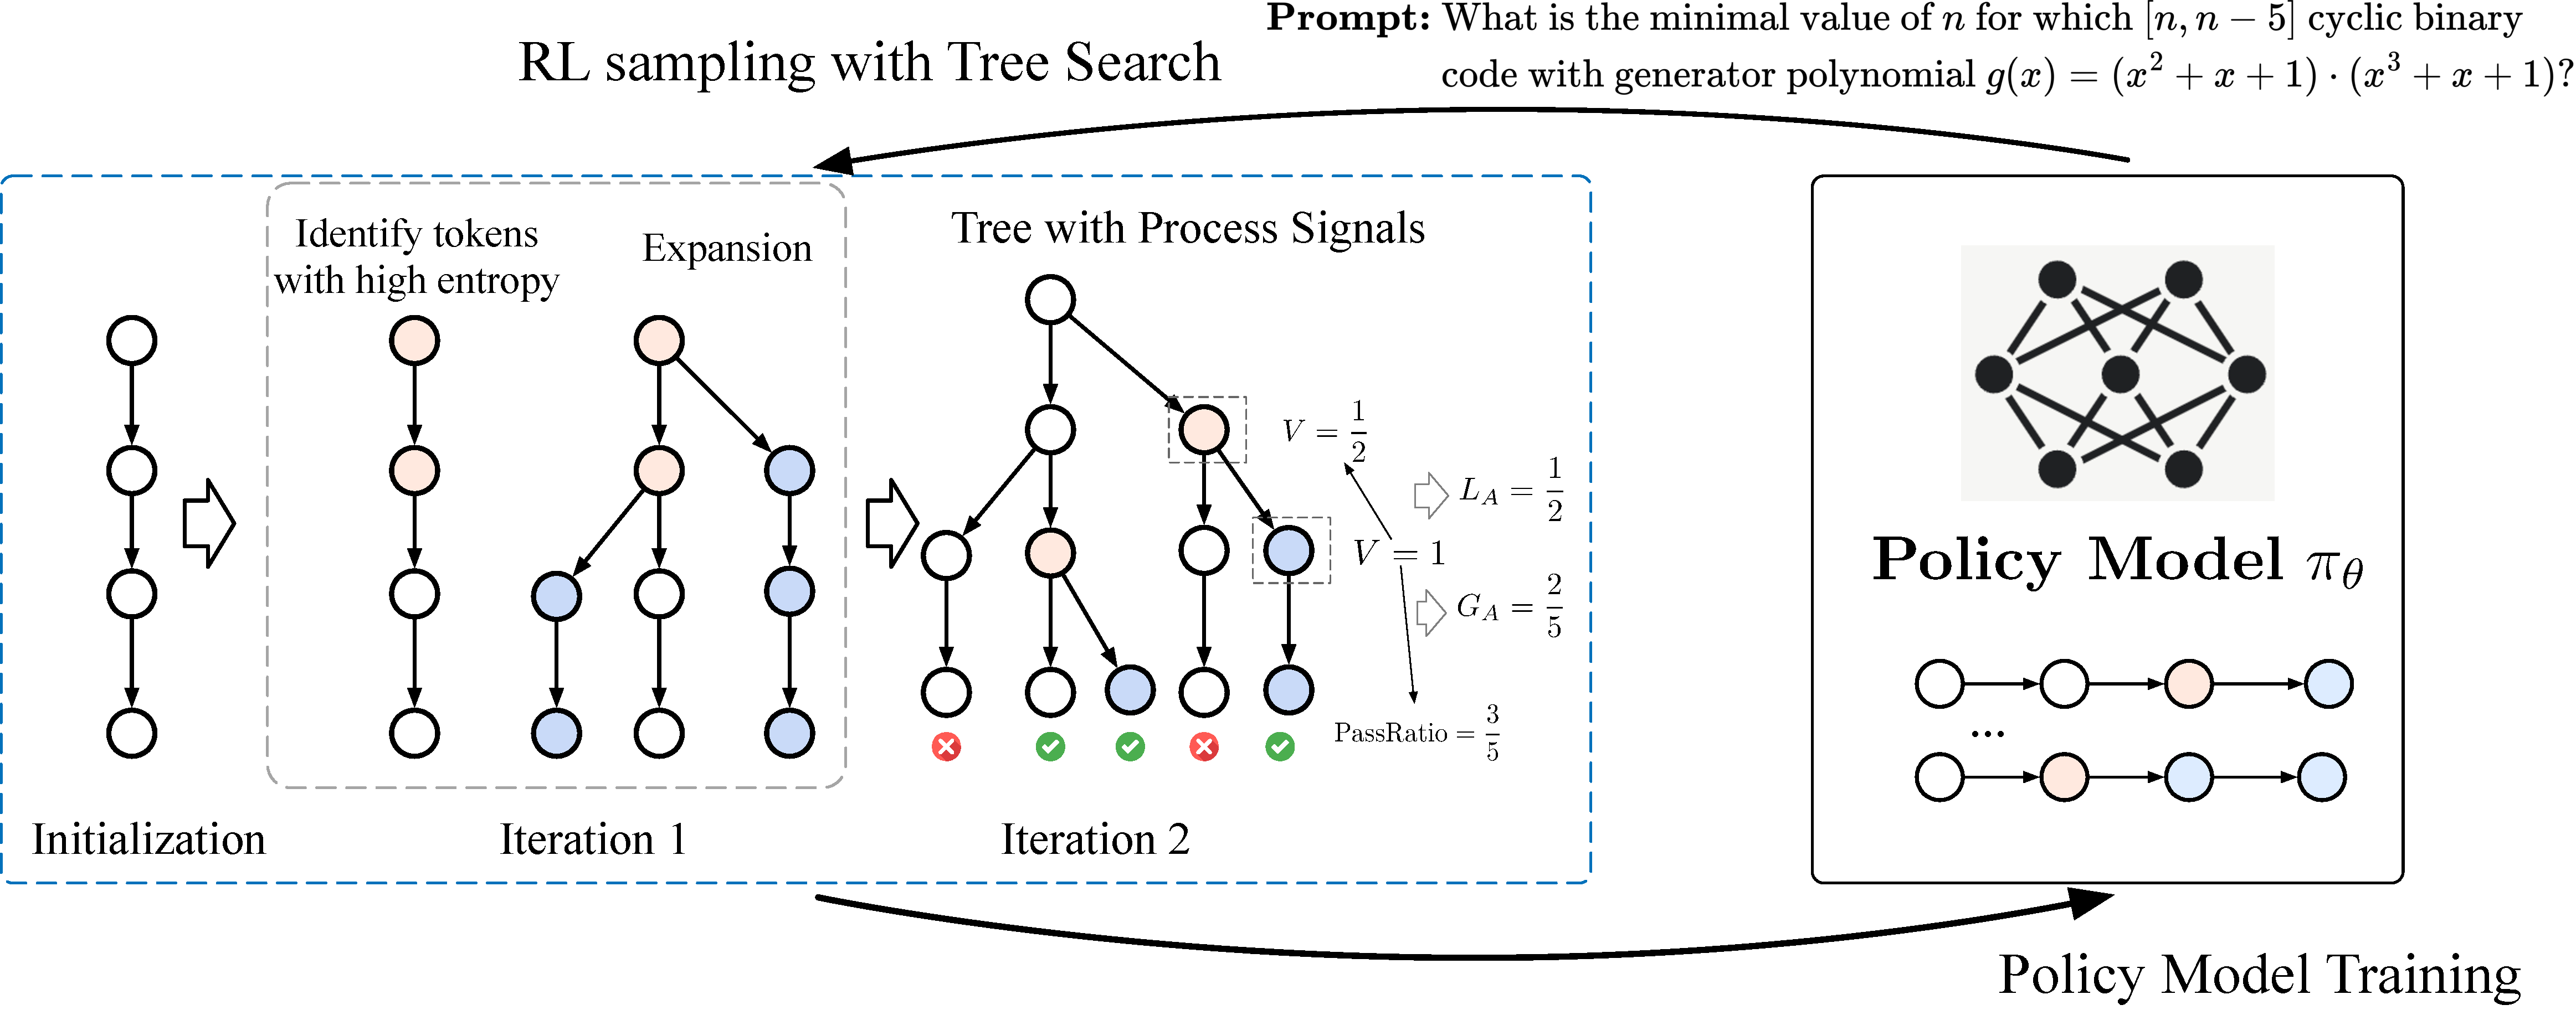
\includegraphics[width=1.0\linewidth]{figure/overview_new.pdf}
    \caption{Illustration of \model. In each iteration, \model first performs a tree search using \treemodel, progressively expanding branches from the top-$N$ most uncertain tokens. The resulting tree, along with the process supervision signals derived from each step, is then fed into reinforcement learning to update the policy model.}
    \label{fig:overview}
\end{figure*}

\section{Preliminary}

% \ziniu{I don't think this part about RLHF is needed given we don't use KL; better to directly define what is so-called chain-RL (iid sampling, / rloo / grpo), what is baseline and value.}
\hide{
To align the fine-tuned model \(\pi_\theta\) with human feedback, \citet{ouyang2022training} proposes to apply reinforcement learning (RL) to enable LLM to learn from self-exploration.
Reinforcement learning maximizes a reward signal, e.g., human preference or final answer correctness, and is accomplished by optimizing the following objective:
\begin{equation}
    % J_r(\pi_\theta) = 
    \underset{\vx \sim p_{\text{data}}, \vy \sim \pi_\theta}{\mathbb{E}} \left[ r(\vx, \vy) - \beta \log \frac{\pi_\theta(\vy \mid \vx)}{\pi_{\text{ref}}(\vy \mid \vx)} \right]
    \label{eq:rl_target}
\end{equation}
where \(r(\cdot)\) is the reward function and assesses the quality or correctness of a response. It takes a prompt \(\vx\) and its response \(\vy\) as input and outputs a scalar reward. \(\pi_{\text{ref}}\) refers to a pre-defined reference model and is used in KL to prevent the policy model from shifting too far from $\pi_{\text{ref}}$.
%\(\pi_{\text{ref}}\) refers to the reference model, often the Supervised Fine-Tuned (SFT) model, and is used to avoid the policy model shifting too far from the reference model.

The typical RL for the LLM process works as follows: for a given prompt \(\vx\), the policy model \(\pi_\theta\) generates \(K\) possible responses, denoted as \((\vy_1, \dots, \vy_K)\). The reward function then assigns a scalar reward to each pair \((\vx, \vy_i)\). Afterward, the policy model \(\pi_\theta\) is updated using reinforcement learning to optimize the objective in \Cref{eq:rl_target}.
}


To align the fine-tuned model \(\pi_\theta\) with feedback signals, \citet{ouyang2022training} proposes to apply reinforcement learning (RL) to enable LLM to learn from self-exploration.
Reinforcement learning maximizes a reward signal, e.g., human preference or final answer correctness.
The typical RL for the LLM process works as follows: for a given prompt \(\vx\), the policy model \(\pi_\theta\) generates \(K\) possible responses, denoted as \((\vy_1, \dots, \vy_K)\). The reward function $r(\vx, \vy_i)$ then assigns a scalar reward to each pair \((\vx, \vy_i)\). Afterward, the policy model \(\pi_\theta\) is updated using reinforcement learning to optimize the following objective:
% , and is accomplished by optimizing the following objective:
\begin{equation}
    % J_r(\pi_\theta) = 
    \underset{\vx \sim p_{\text{data}}, \vy \sim \pi_\theta}{\mathbb{E}} \frac{1}{K} \sum_i^{K}  A(\vx, \vy_i) \log \pi_{\theta}(\vy_i|\vx)
    \label{eq:rl_target}
\end{equation}
where $A(\cdot)$ is the advantage function and usually defined as $A(\vx, \vy_i) = \beta(r(\vx, \vy_i) - b)$, where $b$ is the baseline~\cite{mei2022role,chung2021beyond} and varies in different methods. For example, $A(\vy_i) = \frac{r(\vy_i) - \text{mean}\{r(\vy_i)\}}{\text{std}\{r(\vy_i)\}}$ in GRPO~\cite{shao2024deepseekmath} and $A(\vy_i) = r(\vy_i) - \frac{1}{K-1}\sum_{j\neq i}^K r(\vy_i)$ in RLOO~\cite{ahmadian2024rloo}.
% \(\pi_{\text{ref}}\) refers to a pre-defined reference model and is used in KL to prevent the policy model from shifting too far from $\pi_{\text{ref}}$.



\section{\model: Reinforcement Learning with Tree Search}
In this section, we present \model to improve LLM reasoning with tree search. Figure~\ref{fig:overview} shows the overview of \model. We first present an efficient and effective tree search algorithm \treemodel, which guides tree search by token-level uncertainty instead of traditional Monte Carlo Tree Search (MCTS)~\citep{browne2012mctssurvey}. Then, we show how to integrate the tree search into reinforcement learning with process supervision to improve reasoning capability further.

\subsection{Entropy-Guided Tree Search}
\label{sec:entropy-tree}
We aim to optimize the tree-search algorithm for RL training and thus emphasize the PassRate metric, which evaluates the algorithm's ability to generate diverse yet correct answers under a given inference budget. Furthermore, the tree-search algorithm must be efficient and highly parallelizable. In contrast, traditional MCTS requires numerous iterative generations, making it less efficient in current LLM inference engines like VLLM~\citep{kwon2023efficient}.

% To improve both effectiveness and efficiency in text generation, 
We propose an entropy-guided tree search algorithm, \treemodel.
% , which parallelizes the generation of multiple subtrees.  
The core idea is to iteratively expand the search tree by forking new branches (nodes) from the top-$N$ most uncertain tokens (as measured by entropy) across existing trees.
This encourages exploration in regions of high model uncertainty, leading to improved performance.  
Critically, \treemodel can generate multiple trees in parallel, and the expansion process requires only around 2 iterations to build a diverse and informative tree, making it highly efficient.
The algorithm runs the following steps.

\vpara{Initialization.} To generate $M$ trees in parallel, we first construct \( M \) chains by generating $M$ responses for a given prompt \( \vx \) as initialization of $\mathcal{T}_i$ for further expansion:
\[
Y^{(i)} = \{\vy_i \sim \pi_\theta(\cdot \mid \vx)\},~ \text{for} ~ i = 1, 2, \ldots, M
\]
where \( \pi_\theta \) is the policy model and $\vx$ is the prompt. 

% \subsubsection{Entropy-guided Expansion}

% Next, the trees are iteratively expanded for \( L \) iterations. In each iteration \( l \leq L\), the trees are expanded based on the entropy of the tokens at the leaf nodes. 

\vpara{Forking token selection.} Next, we aim to expand the trees by forking new branches from the existing trees. We propose forking from the tokens with the highest uncertainty, as these tokens provide the most informative signals for the model and encourage exploration.
We use cross-entropy as a measure of uncertainty, which quantifies the uncertainty in the policy model \(\pi_\theta\) when predicting a given token. To promote expansion, the top-\(N\) tokens with the highest entropy values are selected across the whole tree $\mathcal{T}_i$. 
Specifically, the entropy of each token \(v\) in the tree \(\mathcal{T}_i\) is calculated as follows:
\[
B_i = \text{Top-}N_{H(\cdot|\vx)}\left\{\left(t, H\left(\vy_t \mid \vx, \vy_{<t} \right)\right) \mid t \in \mathcal{T}_i\right\}
\]
where \(H(\vy_t) = -\log \pi_{\theta}(\vy_t \mid \vx,\vy_{<t})\) denotes the entropy of token \(\vy_t\). 
% Higher entropy indicates greater uncertainty in the model’s prediction. 
Additionally, we mask tokens near the end of sequences, as the model is expected to explore different reasoning paths rather than simply revisiting previous answers.

% For each token \( v \) in the tree \( \mathcal{T}_i \), we calculate the entropy at each unmasked token position \( t \). 
% "Unmasked positions" refers to the token positions within the sequence that will not be selected for branching.  
% The entropy \( H(y_t) \) at a given position \( t \) quantifies the uncertainty of the language model's prediction for that token, 
% given the preceding tokens \( y_{<t} \) and prompt \( \vx \).  
% This is calculated for all unmasked positions, and those positions with high entropy are the candidate `Forked Points`
% \[
% S_v = \left\{\left(t, H\left(y_t \mid y_{<t}, x\right)\right) \mid t \in \operatorname{Unmasked}(v)\right\}
% \]

% The information entropy \( H(y_t) \) is defined as the negative logarithm of the probability assigned by the model to the token at position \( t \):
% \[
% H(y_t) = -\log \pi_{\theta}(y_t \mid y_{<t}, x)
% \]
% Where $\pi_{\theta}(y_t \mid y_{<t}, x)$ is the probability of token $y_t$ predicted by the model. A higher entropy value indicates greater uncertainty in the model's prediction.

% \( N \) is a hyperparameter that determines the maximum number of branching points in each iteration. 
%These \( N \) positions represent the locations where the model is most uncertain, and therefore, the most promising points to explore alternative generation paths.  
% The set of branching points \( B_l \) for iteration \( l \) is determined as follows:
% \[
% B_l = \operatorname{TopK}\left(\{ S_v \mid  v\in \text{Leaves}(\mathcal{T}_i)\}, N\right)
% \]
% Here,  \(\operatorname{Leaves}(\mathcal{T}_i)\) denotes the set of all leaf nodes in the current tree structure \( \mathcal{T}_i \), and \(\operatorname{TopK}(S, N)\) is a function that returns the \( N \) elements with the highest values from the set. The elements in \( B_l \) are tuples of the form \((v, t)\), indicating the leaf node \( v \) and the token position \( t \) within that node's sequence.

% Each new token is sampled from the language model's conditional probability distribution, given the input context \( x \) and the sequence up to (but not including) position \( t \) in the parent node \( v \), denoted as \( Y_{v,<t} \):
% This means we are asking the language model: "Given the input \( x \) and the sequence up to position \( t \) in node \( v \), what are the probabilities of the next token?" We then sample \( T \) tokens according to these probabilities.  
% For each sampled token \( Y_{\text {new }}^{(j)} \), a new child node is created and appended to the parent node \( v \). The sequence in the new child node is the sequence of the parent node \( v \) up to position \( t \), concatenated with the new sampled token \( Y_{\text {new }}^{(j)} \).  


\vpara{Expansion.} Given the selected tokens for each tree, we continue the generation process from these tokens to form new branches. For each forking point \( t \), with the prefix \( \vy_t \) and prompt \( \vx \), we generate \( T \) different candidate responses until completion:
\[
Y_{\text{new}}^{(i)} \sim \{\pi_\theta\left(\cdot \mid \vx, \vy_{<t}\right), \ \text{for} \ (t,\cdot) \in B_i\}^{T}
\]
where \( \vy_{<t} \) denotes the prefix response before token \( t \). This results in \( M \times N \times T \) tree nodes in total( \(N \times T\) for each tree $\mathcal{T}_i$ ), each corresponding to a new response. The tree structure \( \mathcal{T}_i \) is updated to include these new nodes:
\[
\mathcal{T}_i \leftarrow \mathcal{T}_i \cup Y_{\text{new}}^{(i)}
\]
After initialization, the forking and expansion process is repeated for \( L \) iterations, leading to \( M \times (T \times N \times L+1 ) \) leaves (responses). We denote this entropy-guided tree search as an \( (M, N, L, T) \)-tree, where \( M \) is the number of parallel trees, \( N \) is the number of forked points per iteration, \( L \) is the number of iterations, and \( T \) is the branching factor at each forking point.
% \[
% \mathcal{T}_i \leftarrow \mathcal{T}_i \cup \left\{\operatorname{TreeNode}\left(Y_{v, <t} \oplus Y_{\text {new }}^{(j)}\right)\right\}_{j=1}^T
% \]
% Where $\oplus$ denotes the concatenation operation.

In comparison to independent multi-chain sampling, the \treemodel is capable of producing a larger number of diverse responses under the same inference cost, as illustrated in \Cref{fig:tree_vs_mcts_iid_resp_num}. This offers the potential to enhance RL performance by learning from more varied responses.
% We show that the \treemodel consistently generates more responses than i.i.d. multi-chain sampling under the same inference cost, with the proof provided in the \Cref{sec:appendix:proof}.

\begin{figure}[t]
        \centering
        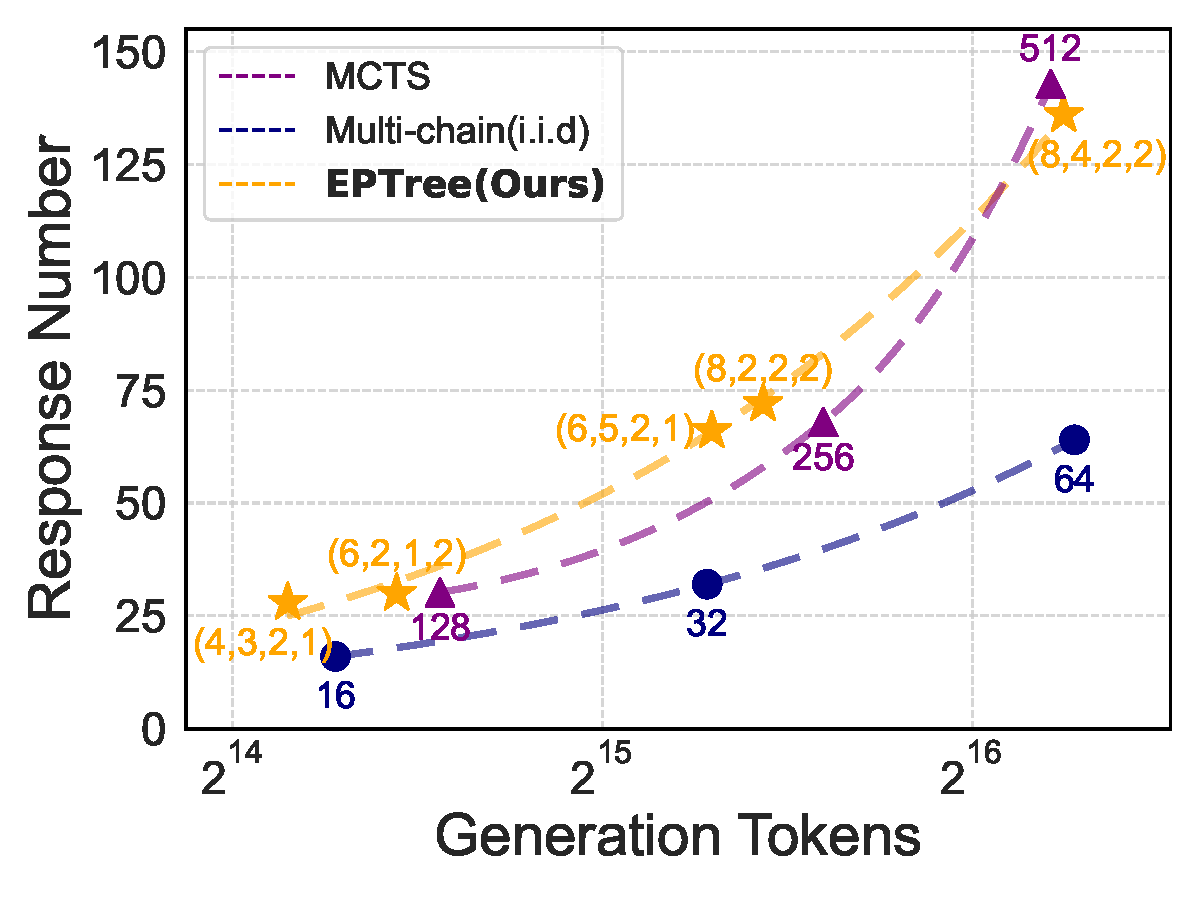
\includegraphics[width=0.45\textwidth]{figure/tree_iid_mcts_leaf_num.pdf}
        \label{fig:tree_vs_iid_leaf_num}
    \caption{Generation diversity comparison of \treemodel, MCTS, and i.i.d. multi-chain sampling. Both \treemodel and MCTS produce approximately $2\times$ different responses compared to i.i.d. multi-chain sampling. }
    \label{fig:tree_vs_mcts_iid_resp_num}
\end{figure}


\begin{algorithm*}[t]
    \caption{\model}
    \label{alg:entropy-guided-tree-search}
    \begin{algorithmic}{}
    \Statex \textbf{Input}: Prompt $\vx$, Policy $\pi_\theta$, Number of Trees $M$, Forking Points $N$, Iterations $L$, Branches $T$
    \Statex \textbf{Output}: Optimized Policy $\pi_{\theta}^*$
        \For{$i = 1$ to $M$} \Comment{\textcolor{blue}{{Create $M$ trees with $M(1+NLT)$ leaves}}}
            \State $Y^{(i)} \leftarrow \{\vy_i \sim \pi_\theta(\cdot \mid \vx)\}$, $\mathcal{T}_i \leftarrow \{Y^{(i)}\}$ \Comment{\textcolor{blue}{{Initialization}}}
            \For{$l = 1$ to $L$} \Comment{\textcolor{blue}{Iterative Expansion}}
                % \State $H(Y_t) = -\log \pi_\theta(Y_t \mid Y_{<t}, \vx), \forall\ Y\in \mathcal{T}_i,t\in\{1,\cdots, |Y|\}$
                \State $H(\vy_t) \leftarrow -\log \pi_{\theta}(\vy_t \mid \vx, \vy_{<t}), \forall\ t \in \mathcal{T}_i$
                % \State $S_v = \{(t, H(Y_t)) \mid t \in \text{Unmasked}(v)\}$
                \State $B_{i, l} \leftarrow \text{Top-}N_{H(\cdot|\vx)}\left\{\left(t, H\left(\vy_t \mid \vx, \vy_{<t} \right)\right) \mid t \in \mathcal{T}_i\right\}$
                % \For{each selected fork $(v, t) \in \operatorname{TopK}(S_v, N)$}
                \For{each selected forking point $(t, \cdot) \in B_{i, l}$}
                    \State $Y_{\text{new}}^{(i,l)} \sim \{\pi_\theta\left(\cdot \mid \vx, \vy_{<t}\right), \ \text{for} \ (t,\cdot) \in B_{i,l}\}^{T}$
                    \State $\mathcal{T}_i \leftarrow \mathcal{T}_i \cup Y_{\text{new}}^{(i,l)}, j\in \{1,\cdots, T\}$
                \EndFor
            \EndFor
        \EndFor
        
        \For{each step $s_n$ in $\mathcal{T}_i$}  \Comment{\textcolor{blue}{Process Reward Calculation}}
            \State $V(s_n) \leftarrow \dfrac{1}{|L(s_n)|} \sum_{l \in L(s_n)} \mathbf{1}(l \text{ is correct})$
            \State $R(s_n) \leftarrow \underbrace{|L(s_n)|^{-1/2}}_{\text{Re-weight Factor}}\cdot [\underbrace{V(s_n) - V(\text{root})}_{\text{\textbf{G}lobal \textbf{A}dvantage}} + \underbrace{V(s_n) - V(p(s_n)}_{\text{\textbf{L}ocal \textbf{A}dvantage}}]$
        \EndFor
    \State Update $\pi_{\theta}$ using RL with process reward by Policy Gradient
    \end{algorithmic}
\end{algorithm*}



\subsection{Reinforcement Learning with \treemodel}
In this part, we show how to integrate \treemodel into RL training.
Beyond the superior potential to find correct trajectories, hierarchical tree structures also provide more fine-grained process supervision for intermediate steps for RL training.

\subsubsection{Process Supervision from Tree Search}
At each step, we estimate the value using Monte Carlo methods.
% and define the process reward from the perspective of advantages. 
Specifically, for a step \( s_n \) (corresponding to a node in the tree), let \( L(s_n) \) denote the set of all leaf nodes that are descendants of node \( s_n \) (including node \( s_n \) itself if it is a leaf). The value \( V(s_n) \) of node \( s_n \) is computed as the ratio of correct leaf nodes among its descendants:
\[
    V(s_n) = \frac{1}{|L(s_n)|} \sum_{l \in L(s_n)} \mathbf{1}(l \text{ is correct})
\]
This value reflects the potential of the node \( s_n \) to lead to correct answers. Based on value, process supervision for each step is defined using advantages, i.e., how much a step is better than other steps, which include both \emph{global} and \emph{local advantages}.

The \emph{global advantage} of a step \( s_n \) represents its potential to lead to a correct outcome compared to the overall correctness ratio of all samples. Without loss of generality, assume that there exists a virtual root node for all subtrees, and the value of the root node $V(root)$ represents the average correctness of all generated responses. The global advantage is then computed as:
\begin{equation}
G_A(s_n) = V(s_n) - V(\text{root})
\label{eq:global_adv}
\end{equation}
% where \( V(s_n) \) denotes the value of node \( s_n \) and \( V(\text{root}) \) represents the value of the root node.
Essentially, the global advantage of \(s_n\) is equivalent to the normalized value, which can be obtained by first normalizing the reward across all leaf nodes---subtracting the average reward---and then calculating the average rewards for \(L(s_n)\).

The \emph{local advantage} of a node \( s_n \) quantifies the improvement the step $s_n$ provides compared to its parent step $p(s_n)$
% its potential relative to its parent node \( p(s_n) \) 
and is defined as:
\begin{equation}
L_A(s_n) = V(s_n) - V(p(s_n))
\label{eq:local_adv}
\end{equation}
where \( V(p(s_n)) \) denotes the value of the node \( p(s_n) \). \( L_A(s_n) > 0 \) indicates that step \( s_n \) is more likely to lead to the correct result than its parent node, suggesting that this step should be encouraged, and vice versa.
% Conversely, \( L_A(s_n) < 0 \) indicates that step \( s_n \) is less likely to lead to a correct outcome than its parent.

To compute the final reward for each step, we combine the global and local advantages as follows:
\begin{equation}
R(s_n) = G_A(s_n) + L_A(s_n)
\label{eq:process_reward}
\end{equation}
% where \( \lambda \) is a hyperparameter and is usually set to 1.
% The global advantage function provides a measure of how each node improves the overall task performance, while the local advantage function quantifies the relative gain contributed by each node in comparison to its parent.

% Inspired by Generalized Advantage Estimation (GAE) by \citet{schulman2015high}, which computes the TD-error by summing over future steps using an exponentially weighted average, we can extend this idea to the supervision process at step \( s_n \). Specifically, we can generalize the process as in \Cref{eq:reward}, by considering not only the root and parent but also all of its ancestor nodes in the trajectory. We assign each ancestor node a weight \( \lambda_j \), and the reward at step \( s_n \) becomes:

% \ziniu{Can we explicitedly write down what's connection? Why the current formula is a special case?}
The definition could be viewed as a special case of Generalized Advantage Estimation (GAE)~\cite{schulman2015high}. The general form of GAE in LLM is defined as:
\begin{equation}
    A(s_n \rightarrow s_{n+t}) = \gamma^t V(s_{n+t}) - V(s_n) 
\end{equation}
where $t$ represents any integer time step, and $\gamma$ is typically set to 1 in most cases. Thus, the local advantage defined in Eq~\ref{eq:local_adv} corresponds to the case where $t=1$, while the global advantage corresponds to the case where $n=0$. 
% Inspired by Generalized Advantage Estimation (GAE)\citep{schulman2015high} in classical RL design, 
% which weights the sum of advantages over all future steps, we extend \Cref{eq:process_reward} to 
Inspired by the GAE, the process supervision signal can be defined as a more generalized format by considering not only the root and direct parent but also all of its ancestor nodes in the trajectory:
% We assign each ancestor node a weight \( \lambda_j \), and the reward at step \( s_n \) becomes:
\[
R_{GAE}(s_n) = \sum_{j \in P(s_n)} \lambda_j \cdot [V(s_n) - V(s_j)]
\]
where \( P(s_n) \) represents the set of ancestor nodes of \( s_n \) and $\lambda_j$ denotes the weight of each step. In this work, we focus on a special format that only considers the direct parent and the root node. 
% In this case, we set \( \lambda_j = \mathbf{1}(j \in \{\text{root}, \text{parent}\}) \), meaning that the weight is 1 if the ancestor is either the root or the parent, and 0 otherwise.

\subsubsection{Training with Process Superivison}
% At each iteration, we first utilize \treemodel described in \Cref{sec:entropy-tree} to generate responses of a given prompt \( \vx \). Specifically, we generate $M$ trees \( \mathcal{T} = \{\mathcal{T}_i\}_i^{M} \) for the prompt, where each leaf node in \( \mathcal{T} \) together with its all prefix corresponds to a complete sequence. 
At each iteration, we first utilize \treemodel described in \Cref{sec:entropy-tree} to generate $M$ trees \( \mathcal{T} = \{\mathcal{T}_i\}_i^{M} \) for the prompt, where each leaf node in \( \mathcal{T} \) together with its all prefix corresponds to a complete sequence. 
% \( seq_i = (a_1, a_2, \ldots, a_k, l_i) \), which spans from the root \( \vx \) to the leaf node \( l_i \). 
For each step in the tree, the process supervision signal is assigned based on \Cref{eq:process_reward} to reflect its importance.

The sequences \(\{ S_1, S_2, \ldots, S_{(M\times N \times L \times T + M)} \} \) extracted from the trees are used for RL training. As all non-leaf steps appear in multiple sequences and will be repeatedly computed in optimization, we downweight the reward of these steps to prevent overfitting. The reward for each non-leaf step is modified by dividing the square root of the number of leaf nodes in its subtree: \( R(s_n) = R(s_n) / \sqrt{|L(s_n)|} \). This adjustment leads to improved performance in our experiments. The overall pipeline of \model is illustrated in Alg~\ref{alg:entropy-guided-tree-search}.


